%%%%%%%%%%%%%%%%%%%%%%%%%%%%%%%%%%%%%%%%%%%%%%%%%%%%%%%%%%%%%%%%%%%%%%%%%%%%%%%
%                       CARREGA DE LA CLASSE DE DOCUMENT                      %
%                                                                             %
% Les opcions admissibles son:                                                %
%      12pt / 11pt            (cos dels tipus de lletra; no feu servir 10pt)  %
%                                                                             %
% catalan/spanish/english     (llengua principal del treball)                 %
%                                                                             % 
% french/italian/german...    (si necessiteu fer servir alguna altra llengua) %
%                                                                             %
% listoffigures               (El document inclou un Index de figures)        %
% listoftables                (El document inclou un Index de taules)         %
% listofquadres               (El document inclou un Index de quadres)        %
% listofalgorithms            (El document inclou un Index d'algorismes)      %
%                                                                             %
%%%%%%%%%%%%%%%%%%%%%%%%%%%%%%%%%%%%%%%%%%%%%%%%%%%%%%%%%%%%%%%%%%%%%%%%%%%%%%%

\documentclass[11pt,spanish,listoffigures,listoftables]{tfgetsinf}

%%%%%%%%%%%%%%%%%%%%%%%%%%%%%%%%%%%%%%%%%%%%%%%%%%%%%%%%%%%%%%%%%%%%%%%%%%%%%%%
%                     CODIFICACIO DEL FITXER FONT                             %
%                                                                             %
%    windows fa servir normalment 'ansinew'                                   %
%    amb linux es possible que siga 'latin1' o 'latin9'                       %
%    Pero el mes recomanable es fer servir utf8 (unicode 8)                   %
%                                          (si el vostre editor ho permet)    % 
%%%%%%%%%%%%%%%%%%%%%%%%%%%%%%%%%%%%%%%%%%%%%%%%%%%%%%%%%%%%%%%%%%%%%%%%%%%%%%%
\usepackage[utf8]{inputenc} 
%%%%%%%%%%%%%%%%%%%%%%%%%%%%%%%%%%%%%%%%%%%%%%%%%%%%%%%%%%%%%%%%%%%%%%%%%%%%%%%
%                        ALTRES PAQUETS I DEFINICIONS                         %
%                                                                             %
% Carregueu aci els paquets que necessiteu i declareu les comandes i entorns  %
%                                          (aquesta seccio pot ser buida)     %
%%%%%%%%%%%%%%%%%%%%%%%%%%%%%%%%%%%%%%%%%%%%%%%%%%%%%%%%%%%%%%%%%%%%%%%%%%%%%%%

%\usepackage[13-19]{pagesel}

\newenvironment{no_desc}{
   \begin{itemize}
      \setlength{\itemsep}{0.2pt}
}{\end{itemize}}

%%%%%%%%%%%%%%%%%%%%%%%%%%%%%%%%%%%%%%%%%%%%%%%%%%%%%%%%%%%%%%%%%%%%%%%%%%%%%%%
%                        DADES DEL TREBALL                                    %
%                                                                             %
% titol, alumne, tutor i curs academic                                        %
%%%%%%%%%%%%%%%%%%%%%%%%%%%%%%%%%%%%%%%%%%%%%%%%%%%%%%%%%%%%%%%%%%%%%%%%%%%%%%%

\title{Guía para la definición y adaptación de algoritmos para su implementación 
en FPGAs mediante High Level Synthesis}
\author{Víctor Juan Quevedo}
\tutor{David De Andres Martinez}
\curs{2020-2021}

%%%%%%%%%%%%%%%%%%%%%%%%%%%%%%%%%%%%%%%%%%%%%%%%%%%%%%%%%%%%%%%%%%%%%%%%%%%%%%%
%                     PARAULES CLAU/PALABRAS CLAVE/KEY WORDS                  %
%                                                                             %
% Independentment de la llengua del treball, s'hi han d'incloure              %
% les paraules clau i el resum en els tres idiomes                            %
%%%%%%%%%%%%%%%%%%%%%%%%%%%%%%%%%%%%%%%%%%%%%%%%%%%%%%%%%%%%%%%%%%%%%%%%%%%%%%%

\keywords{HLS, Xillinx, C/C++, Algorismes, FPGA, Vivado/Vitis} % Paraules clau 
         {HLS, Xillinx, C/C++, Algoritmos, FPGA, Vivado/Vitis} % Palabras clave
         {HLS, Xillinx, C/C++, Algorithms, FPGA, Vivado/Vitis} % Key words

%%%%%%%%%%%%%%%%%%%%%%%%%%%%%%%%%%%%%%%%%%%%%%%%%%%%%%%%%%%%%%%%%%%%%%%%%%%%%%%
%                              INICI DEL DOCUMENT                             %
%%%%%%%%%%%%%%%%%%%%%%%%%%%%%%%%%%%%%%%%%%%%%%%%%%%%%%%%%%%%%%%%%%%%%%%%%%%%%%%

\begin{document}

%%%%%%%%%%%%%%%%%%%%%%%%%%%%%%%%%%%%%%%%%%%%%%%%%%%%%%%%%%%%%%%%%%%%%%%%%%%%%%%
%              RESUMS DEL TFG EN VALENCIA, CASTELLA I ANGLES                  %
%%%%%%%%%%%%%%%%%%%%%%%%%%%%%%%%%%%%%%%%%%%%%%%%%%%%%%%%%%%%%%%%%%%%%%%%%%%%%%%

\begin{abstract}

\end{abstract}

\begin{abstract}[spanish]

\end{abstract}

\begin{abstract}[english]

\end{abstract}

%%%%%%%%%%%%%%%%%%%%%%%%%%%%%%%%%%%%%%%%%%%%%%%%%%%%%%%%%%%%%%%%%%%%%%%%%%%%%%%
%                              CONTINGUT DEL TREBALL                          %
%%%%%%%%%%%%%%%%%%%%%%%%%%%%%%%%%%%%%%%%%%%%%%%%%%%%%%%%%%%%%%%%%%%%%%%%%%%%%%%

\mainmatter

%%%%%%%%%%%%%%%%%%%%%%%%%%%%%%%%%%%%%%%%%%%%%%%%%%%%%%%%%%%%%%%%%%%%%%%%%%%%%%%
%                                  INTRODUCCIO                                %
%%%%%%%%%%%%%%%%%%%%%%%%%%%%%%%%%%%%%%%%%%%%%%%%%%%%%%%%%%%%%%%%%%%%%%%%%%%%%%%

\chapter{Introducci\'on}

   En 1984, Ross Freeman ingeniero estadounidense el\'ectrico y Bernard Von Der
   Schmitt, los dos cofundadores de Xillinx, inventaron la FPGA, como resultado
   de la uni\'on de diversas tecnologías y evolución de los CPLD, situando a
   Xillinx como marca m\'as populares en el desarrollo de esta tecnología, que
   actualmente podemos encontrar en diversos sectores, como el sector
   automovilístico, médico o big data, por su amplio rango de aplicaci\'on.    
   
   Actualmente esta tecnología juegan un papel importante en determinadas tareas
   dedicadas, ya que ofrecen un mayor rendimiento que las CPU's tradicionales.
   Esto ha hecho que la FPGA sufra un crecimiento en los últimos a\~{n}os, pero
   el desarrollo en estas necesita de conocimientos específicos en dise\~{n}o de
   sistemas digitales y adaptarse a los lenguajes de descripción, como VHDL o
   Verilog.

   A consecuencia de este crecimiento experimentado las distintas marcas
   dedicadas al desarrollo de estas tecnolog\'ias crearon herramientas de
   desarrollo en lenguajes de alto nivel para resolver este problema y as\'i
   mejorar la gesti\'on del dise\~{n}o y el crecimiento de la productividad en
   el campo del desarrollo de software para esta, High Level Synthesis o HLS, el
   cual aplica una capa de abstracción en el proceso de desarrollo. El HLS se
   encarga de interpretar la descripci\'on de estos lenguajes que despu\'es
   usara para la creaci\'on de un sistema digital, el cual implementara el
   comportamiento descrito mediante m\'aquinas de estado finito.
   
   Y aunque utilizar el high level synthesis conlleva un aprendizaje de todas sus
   metodologías, directivas o librerías, serán mucho m\'as familiares y cercanas
   al desarrollo en lenguajes de alto nivel. Así pues, la necesidad de tener un
   alto rango de conocimientos sobre esta tecnología, disminuye y hace que el
   mundo de las FPGA m\'as accesible a los desarrolladores, ya que solo necesitan
   como mínimo conocimientos de C/C++ y acatar unas normas de estilo de c\'odigo.

\newpage{}
\section{Motivaci\'on}
\section{Objetivos}

   Como objetivo principal se pretende llegar a explicar las caracteristicas del
   High Level Synthesis desarollado por Xillinx por tal de poder definir una
   guia/pautas para la definición e implementación de algoritmos escritos en
   C/C++, asi finalmente poder adaptar un algoritmo dedicado para el
   funcionamiento en CPU's, a un algoritmo sintetizable y funcional en una FPGA.
   
   Para ello el objetivo principal esta subdividido en tres partes a conseguir:
   \begin{itemize}
      \item Desarollar una primera version sintetizable, la cual se centra en
      encontrar las diferentes restricciones propuestas por el HLS de Xillinx.
      \item Desarollar una version optimizada del problema, la cual se subdivide
      en dos partes:
      \begin{itemize}
         \item Desarollo de una version con las directivas \#pragma para mejorar
         accesos a array o recorridos de estos.
         \item Desarollo de una version con librerias propias del HLS para
         optimizar los recursos usados.
      \end{itemize}
      \item Desarollo de la version final, la cual incluye todo lo tratado
      anteriormente y comparar las difernetes versiones con esta version, para
      ver hasta que punto mejora.  
   \end{itemize}

\section{Impacto esperado}

   Actuamente el uso de las FPGA crece, ya que estas son perfectas en algunos
   campos en que el coste/computacion es crucial. Por otra parte incorporarse en
   este mundo, y aunque con la aparicion del los HLS facilite mucho mas esto, no
   deja de ser necesario tener ciertos conocimientos y metodologías para llegar
   a tener un codigo util y sintetizable.  Por tanto con este trabajo se espera
   acercar lo maximo posible el HLS y facilitar la incorporacion a esta mediante
   una guia/pautas que ayudaran a entender el comportamiento de esta y asi poder
   empezar de zero mas facilmente.

\section{Estructura de la mem\'oria}

\section{ODS}


%\section{Notes bibliografiques} %%%%% Opcional

%????? ????????????? ????????????? ????????????? ????????????? ?????????????

%%%%%%%%%%%%%%%%%%%%%%%%%%%%%%%%%%%%%%%%%%%%%%%%%%%%%%%%%%%%%%%%%%%%%%%%%%%%%%%
%                         CAPITOLS (tants com calga)                          %
%%%%%%%%%%%%%%%%%%%%%%%%%%%%%%%%%%%%%%%%%%%%%%%%%%%%%%%%%%%%%%%%%%%%%%%%%%%%%%%
\chapter{Estado de arte}

   Actualmente experimentamos un crecimiento tecnologico con aplicaciones de
   cierta complejidad y costo computacional, donde las CPU's tradicionales no
   puede cubrir, ya que estas tienen tiempos de latencias altos a comparacion de
   las FPGA, y no podriamos cubrir la necesidad de una respuesta con un corto
   periodo de tiempo.
   
   Por otra parte algunas de las tareas se suelen atribuirse a GPUs gracias a su
   capacidad de llevar a cabo operaciones de computo en paralelo, situando a las
   GPUs a ser el refuezo mas popular a la hora de realizar operaciones
   matematicas costosas. No obstante esta popularidad ganada, no se debe a una
   superioridad en computo sobre las FPGAs, sino por su facilidad a la hora de
   configurar estas, ya que funcionan a partir de intrucciones que que son
   interpretadas por la CPU, haciendo que su configuracion se base en lenguajes
   de programacion más comunes como C/C++, Python, Java, mientras que las FPGA
   requieren de conocimientos mucho mas específicos sobre la tecnologia para
   configurarlas a partir de lenguajes de descripcion VHDL y Verilog.   Todo
   esto dejo a la FPGA en un papel secundario en este tipo de aplicaciones y
   priorizar a metodos como la parelizacion mediante las GPUs como un recurso
   mucho mas valorado incluso actualmente. Esta situacion llevo a valorar nuevas
   formas de configurar las FPGAs, dando paso al High Level Synthesis, una
   tecnologia que cambia completamente el flujo de diseño en la FPGAs, lo que
   conllevo a un desarollo mucho mas versatil y preciso. 
   
   En la actualidad encontramos varias de estas herramientas de HLS, promovidas
   por diferentes marcas como Intel con Intel High Level Synthesis Compiler o
   Xillinx con VitisHLS, siendo esta ultima la herramienta analizada utilizada
   en el trabajo presente.
   
   El VitisHLS funciona dando como entrada en C/C++ sintetizable con su
   funcionamiento ya verificado, y esta a partir de la entrada construira un
   circuito funcional ya configurado. No obstante este son los pasos minimos en
   el flujo de diseño, ya que entre ellos encontramos varias configuraciones de
   optimizacion en el entrada de codigo para manipular las diferentes entradas
   en el RTL o disminiuir el numero de bloques usados.

   
\chapter{FPGA}

  Dentro del mercado de los circuitos integrados encontramos varios tipos de
  dispositivos, abarcando desde circuitos electronicos diseñados expresamente
  para la problematica a dispositivos reprogramable que se adaptan en funcion de
  las necesidades. Dentro de las reprogramables encontramos la tecnologia FPGA o
  Field Programmable Gate Array conformada por diversos bloques logicos
  configurables que pueden ser modificables dependiendo la necesidad del diseño,
  dando como resultado un crecimiento en diferentes sectores de la industria por
  sus caracteristicas.
  
  Cuanto a su configuración, estas utilizan lenguajes de descripción para
  implementar un diseño, normalment estos lenguajes suelen ser
  VHDL o Verilog que se encargan de dar las intrucciones necesarias para la
  creación de microarquitecutras que son transferidos a la FPGA mediante el un
  proceso que genera un archivo Bitstream. Una vez generado, el Bitstream 
  contiene todo lo necesario para configurar la FPGA, la logica descrita, las
  rutas para llegar a los bloques logicos y los valores iniciales. 
  
  Si profundizamos en la arquitectura, esta se compone principalmente de bloques
  logicos o CLB, los cuales esta interconectados dependiendo del comportamiento
  descrito por el Bitstream. No obstante esta aun necesitan de una forma de
  comunicar su logica con el exterior de la FPGA y aqui entran en juego la
  celdas de entrada y salida o IOB. Finalmente con el enrutado de los CLBs y los
  IOBs obtenmos una matriz de enrutado que puede ser reprogramada, otrogando a
  la FPGA una gran flexibilidad en cuando a las especifiaciones del diseño, lo
  que permite evoluciónar a la par con la problematica encargada de tratar.

  \begin{figure}[h]
   \centering
   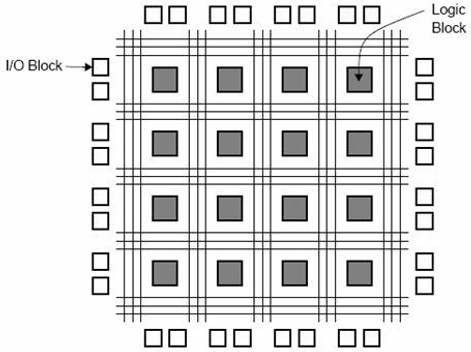
\includegraphics[width=8cm]{img/fpga-chapter/fpga_introduction.png}
   \caption{Arquitectura FPGA simplificada}
   \label{fig:fpga_arch}
  \end{figure}

\section{Arquitectura de la FPGA}

  Como se ve en \ref{fig:fpga_arch}, la arquitectura de una FPGA consiste en
  varios arreglos de CLB interconectados mediante cananales de direccion
  horizontal y vertical, lo que conforma una matriz y aunque esta tecnologia
  pueda variar en sus bloques logicos y la forma de enrutarlos, esto solo
  dependera del fabricante, por tanto en este apartado dedicaremos a resumir la
  arquitectura de la FPGA desde el punto mas general dentro de su arquitectura
  mas regular.

  \subsection{Cofigurable Logic Block}
      Los bloques logicos son los que implementan las funciones logicas a
      necesidad del diseño y estan compuestos por diferentes componenetes para
      despeñar la funcion necesaria. El numero componenetes de estos pueden
      variar dependiendo de las caracteristicas del CLB, pero en general
      consiste en una o varios LUT's cuyas salidas se encuentran multiplexadas y
      son tratadas dependiendo de unos parametros de configuracion del CLB.

      \begin{figure}[h]
         \centering
         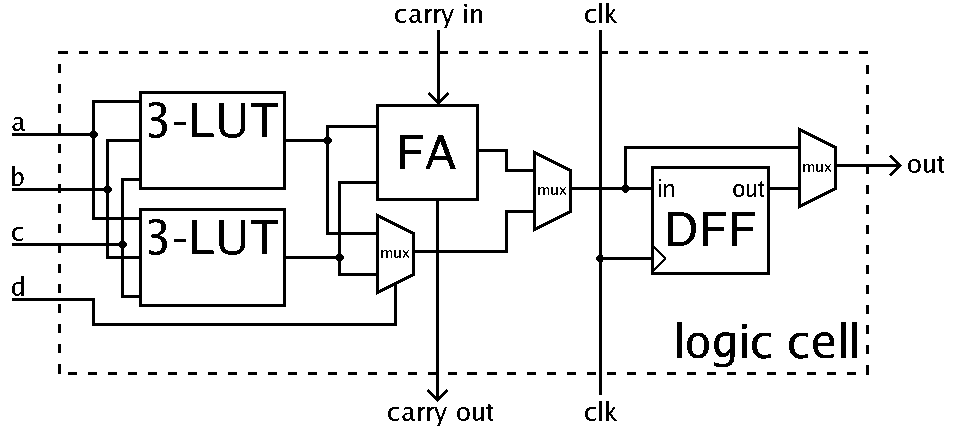
\includegraphics[width=8cm]{img/fpga-chapter/FPGA_cell_example.png}
         \caption{Estructura general de un bloque logico}
         \label{fig:clb_arch}
      \end{figure}

      Su arquitectura mas general, como podemos ver en \ref{fig:clb_arch}, se
      compone de:

      \begin{itemize}
         \item \textbf{Look-up tables:} Esta determina una salida a partir de
         una tabla y por tanto ser\'a la que describa el comportamiento logico,
         no obstante el tamaño de esta variara dependiendo de las
         caracteristicas necesarias.  

         \item \textbf{Full adder:} El Full Adder se caracteriza por ser una
         unidad aritmetologica, la cual tiene un amplio uso en el sistema con
         operaciones tipo suma, resta, multiplicacion, division o como contador.
         
         \item \textbf{Flip-Flop tipo D:} De toda la familia existente de los
         biestables, este tipo suele ser útil cuando hablamos de almacenar
         información, no obstante esta informacion será unicamente un bit.

      \end{itemize}

      Finalmente el numero de elementos dentro del bloque logico dependera sobre
      todo, de las caracteristicas del producto y del proposito al que quermos
      llegar, por ejemplo en la eleccion de entradas de las LUT, la cual sera
      mas  lenta, pero mejor optimizaran el area de uso cuanto menor numero de
      entradas tenga, mientras que a mayor numero de entradas estas permiten
      realizar operaciones mas complejas a cambio de usar mas area.

  \subsection{Input/Output Block}
  
      Esta es la parte encargada de comunicar la FPGA con el exterior y por
      tanto podrán tanto como enviar o recibir señales o realizar las dos
      acciones. Los bloque IOB's son bloques que tiene un alto rango de
      adaptabilidad al poder trabjar con distintas tensiones o estandares
      digitales, haciendo que la FPGA pueda adaptarse comodamente a las
      necesidades.  Cuanto a su numero, existe un bloque de estos por cada
      terminal de I/O del FPGA, lo que posibilita la configuracion independiente
      de cada terminal y la existencia de un buffer unico para cada uno de
      ellos.

  \subsection{Block Random Access Memory}
      
      Los bloques de RAM, son elementos dedicados al almacenado de datos y como
      su propio nombre indica, la encontramos en forma de bloques. Estos bloques
      son bastante flexibles y se adaptan a las necesidades del diseño pudiendo
      configura estos como memoria RAM, ROM o FIFO.
      
      La BRAM es compuesta en parte por LUT's, ya que estas como se ha comentado
      anteriormente contienen tablas de consulta, convirtiendola en una pequeña
      unidad de almacenamiento, la cual se configura al inicio de la ejecucion.
      Dotando a la BRAM de pequeñas memorias muy rapidas, no obstante estas al
      igual que la RAM tradicional, para acceder a ellas se necesitara la ruta
      donde se encuentra.
      
      \begin{figure}[h]
         \centering
         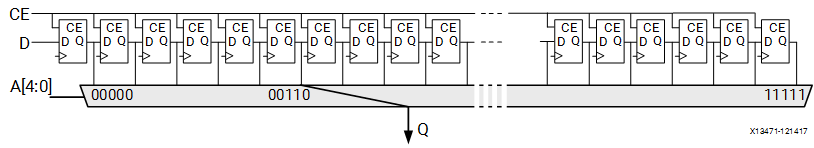
\includegraphics[width=8cm]{img/fpga-chapter/shiftRegister.png}
         \caption{Estructura de un registro de desplazamientos}
         \label{fig:shift_register}
      \end{figure}
         
      El papel del enrutado en estas memorias es dado a las estructuras de
      desplazamiento de registros, donde encontramos al igual que un CLB un
      numero de Flip-Flops tipo D, lo cual dependerá de la grandaria de la
      memoria. Dotando estas a la memoria BRAM una logica computacional para
      encontrar la ruta del LUT dentro del bloque.

  \subsection{Enrutado}

      Los enrutados son los encargados de conectar las distintas logicas entre
      si, creando los difernetes caminos para llegar a los diferentes bloques.
      Las conexiones entre si esta hechas mediante varios canales, no obstante
      entre para efecutar la conexion entre ellos encontramos un nuevo tipo de
      bloque, en este caso los bloques  de conexiones.
      
      \begin{figure}[h]
         \centering
         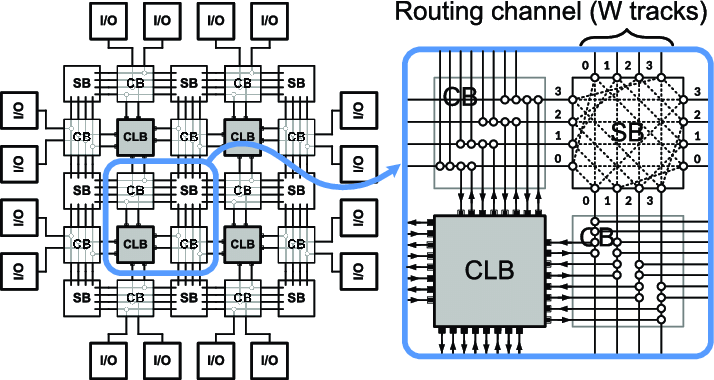
\includegraphics[width=8cm]{img/fpga-chapter/routing.png}
         \caption{Estructura simplificada del enrutado en una FPGA}
         \label{fig:routing_fpga}
      \end{figure}

      Estos bloques contienen diferentes inputs, siendo estos los encargados de
      redirigir el output mediante la ruta indicada para llegar al siguiente
      bloque, ya sea otro bloque de conexion o los tratados anteriormente. No
      obstante, como se puede ver en la imagen \ref{fig:routing_fpga} dentro de
      los bloques de conexiones encontramos swiches, que son los encargados de
      guiar la señal por dentro del bloque de conexiones.

\section{Arquitecturas heterogenias}
   Con el tiempo la necesidad de adaptabilidad en los diseños gana importancia,
   ya que en la actualidad las nuevas tecnologias se incorporan a la vida
   diaria.  Esto ha dado como resultado una cantidad de nuevas tecnologias
   diseñadas para suplir esta necesidad, llegando a encontrar distintas
   tecnologias en varios sectores, donde las distintas arquitecturas son
   implementadas por el diseñador segun el proposito y coste de esta.  

   Dependiendo de la arquitectura encontramos, diseños creados expresamente para
   la problematica, diseños dirigidos a ser altamente configurable y flexibles
   con el cambio o diseños que intenta incorporar ambos en cierta medida a
   cambio de sacrificar otras caracteristicas. Algunas de estas arquitecturas
   son:

   \subsection{CPU}
      Actualmente esta es la arquitectura mas conocida y la mas antigua de todas
      las que comentaremos. Su trabajo principalmente es la coordinacion de los
      diferentes elementos que conforman actualmente una computadora, lo que nos
      lleva a encotrar varios tipos dependiendo, del mercado al que vayan
      destinado y se componen por un unico circuito integrado o varios CPU's en
      un mismo circuito como es el caso de los procesadores multinucleo.

      Este funciona a base de la interpretacion de intrucciones, para realizar
      las diferentes acciones ya sean, operaciones aritmeticas, manipurlacion de
      registros, deconficacion de estas mismas intrucciones etc. Cuanto a su
      arquitectura mas simple, se compone de:
      
      \begin{itemize}
         \item \textbf{Registro internos:} Encargada de guardar los distintos registros,
         tanto los accesibles, como los no accesibles.
         \item \textbf{Unidad aritmetico logica:} Como su nombre indica realiza las
         operaciones aritméticas y lógicas.
         \item \textbf{Unidad de control:} Se encarga de dirgir la informacion entre los
         registros de la CPU, seguidamente esta conecta con la unidad aritméto
         lógica las intrucciones que se han extraido.
      \end{itemize}

   \subsection{GPU}

      Juntamente con la unidad central de procesamiento, esta es una de las
      tecnologias mas populares actualmente y aunque pueda llegar a ser similar,
      esta tiene diferentes propositos y funcionamientos, los cuales en un
      principio fuero mostrar por pantalla graficos hasta ahora, las cuales son
      buscadas para el procesamiento paralelo.

      La arquitectura de la GPU a dia de hoy se encuentra segmentada con
      multiples nucleos optimizados para la ejecucion de procesos en paralelo.

   \subsection{ASIC}

     Dentro de todas las arquitecturas desarolladas en este capitulo, esta es la
     unica la cual esta hecha para una tarea especifica y no esta pensada para 
     propositos generales. Como arquitectura encontramos varios diseños:

      \begin{itemize}

         \item \textbf{Dise\~{n}o basado en Celdas Estándares:} El diseño ASIC
         basado en celdas estandares, se caracteriza por tener su celdas logicas
         como puertas logicas multiplexores o flip-flops ya prediseñadas por los
         diseñadores de la propia ASIC, lo que con lleva a tener diferentes
         configuraciones guardadas en forma de librerias. Esto se conoce como
         "standard cell library".

         \begin{figure}[h]
            \centering
            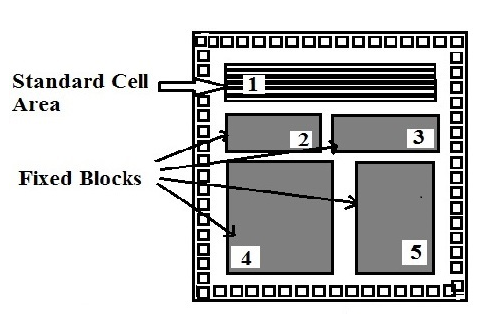
\includegraphics[width=8cm]{img/fpga-chapter/standar_cell.png}
            \caption{Diseño basado en Celdas Estándares}
            \label{fig:standard_cell}
         \end{figure}

         Este diseño ASIC, como se puede ver en \ref{fig:standard_cell}, esta
         compuesto por dos componentes con propositos generales, primeramente
         encontramos la celda estandar es un bloque organizado en celdas
         estandarizadas en filas y su funcionamiento dependera de las "standar
         cell libraries". Por otra parte encontramos los bloque fijos o C-BIC,
         estos son capas customizadas donde el diseñador puede colocar otras
         celdas estandares.
         
         \item \textbf{Diseño basado en Matriz de Puertas:} En este diseño, la placa
         ASIC, viene predefinida por un numero de transistores en una oblea de
         silicio, en esta el diseñador no puede cambiar el lugar donde se alojan
         estos. Esto acaba formando pequeños patrones repetitivos de "base
         array", los cuales son patrones de matrizes logicas donde la
         interconexion de estas, es donde el diseñador tiene la responsabilidad
         de conectar usando capas de metal y asi obtener el funcionamiento
         logico deseado. 

         Dentro del diseño basado en Matrizes de Puertas, encontramos tres tipos:

         \begin{itemize}
            \item{\textbf{Channeled Gate Array:}} Se caracteriza por tener un espacio
            fijos entre filas de transistores.

            \item{\textbf{Channel Less Gate Array:}} Al contrario que en el diseño
            comentado anteriormente, no deja espacio libre para el enrutado de los
            transistores. Por tanto el enrutado pasara a ser un enrutado
            personalizado entre el metal y el transistor.

            \item{\textbf{Structured Gate Array:}} A diferencia de los otros tipos de
            estructuracion, que principalmente se centraban en la interconexion de
            los transistores, se centra en integrar tambi\'en un bloque y asi poder
            tener bloques configurables en el diseño. 
         \end{itemize}
         
         \item \textbf{Diseño ''Full Custom'' o hecho a medida:} El diseño ''Full Custom'',
         esta destinado a una acción en específica y por tanto todas sus
         interconexiones y capas son personalizadas para la problematica a
         tratar. Esto conlleva a que el propio diseñador no pueda cambiar la
         interconexion de estos, ya que sino obtendriamos un resultado diferente
         al dado, haciendo que el diseñador se centre enteramente la optimización
         de este, construyendo distintos circuitos o optimizando las celdas de
         memoria.

      \end{itemize}

\section{FPGA vs Otras tecnologias}
   Cuando hablamos de FPGA, podemos destacamos ciertas caracteristicas y las
   comparamos con otras arquitecturas para llegar a saber cual nos interesa más
   para el problema a tratar. Algunos de los detalles a comparar con otras
   arquitecturas de las detalladas anteriormente són:

   \subsection{Rendimiento}
      A terminos de rendimiento, esto siempre dependerá de la necesidad a
      tratar, ya que si nos decantampos por procesos que siguen una esquematica
      muy secuencial, claramente las CPU, serán mas aptas para este tipo de
      tareas. No obstante, cuando queramos el mayor rendimiento en calculo o
      procesamiento en paralelo, nos decantaremos por tecnologias como la GPU,
      la FPGA o el ASIC y por tanto podran ejecutar estas funciones más rápido.
      
      Por otra parte, como hemos mencionado anteriormente las GPU, FPGA y ASIC
      estan mas enfocadas para el procesamiento o calculo paralelo, pero cuanto
      a rendimiento los diseños de ASIC y FPGA serán más rápidas, ya que la GPU
      dependera sustancialmente de la interacción con la  CPU. Y en cuanto a
      mayor rendimiento entre la tecnologia ASIC y FPGA, la tecnologia ASIC
      mostrara mejor rendimiento, ya que la FPGA sacrifica un poco de este a
      cambio de otras caracteristicas que comentaremos seguidamente.

   \subsection{Programabilidad}

      Esta caracteristica hace que el diseño obtenido pueda llegar a ser
      reconfigurable y a su vez pueda ser adaptable al cambio, por tanto la
      tecnologia ASIC es la mas perjudicada, ya que como hemos comentado
      anteriormente esta se basa en diseños hecho a medida para la tarea a
      tratar. Sin embargo las GPU y CPU son las mas beneficiadas por su
      configuracion a bases de instrucciones, lo que permite configurarlas con
      con más facilidad. Mientras que la tecnologia FPGA como se ha comentado
      anteriormente, esta sacrifica rendimiento a cambio de mejorar en el
      aspecto de Programabilidad.  No obstante, esta sigue llegando a ser
      complicada, ya que hay que tener un alto conocimiento sobre el diseño y
      configirarla a base de maquina de estados.

   \subsection{Adaptabilidad}

      Cuanto adaptabilidad las CPU, GPU y FPGA son superiores en esta aspecto
      por ser reconfigurables, lo que permite ser mas flexibles frente los
      cambios y adaptarse a ello cos que con un dispositivo ASIC solo
      conseguiriamos mediante el rediseño de este.

   \subsection{Coste/Eficiencia}

     Cuando hablamos de coste a partir de Eficiencia, siempre se intenta hacer
     un estudio del caso a tratar, ya que dependiendo de las caracteristicas del
     problema a tratar podemos acabar utilizando un sistema empotrado para
     tareas donde el procesamiento sea secuencial y la necesidad de cores no sea
     de extrema necesidad. Mientras que si necesitamos una respuesta rapida
     mediante un cambio, como podria ser la conduccion autonoma, el uso de ASIC
     o FPGA frente la GPU es preferible, ya que estas no cuentan con tantos
     procesos intermedio y necesitariamos mas GPU's para llegar a suplir la
     necesidad, haciendo que el coste se dispare por ende el estas dos serian
     perfectas para esto. Sin embargo entre estas dos el ASIC puede llegar a ser
     muy eficiente pero al tiempo habria que rediseñarla haciendo la un proceso
     mucho mas caro, un punto donde la FPGA no necesitaria ya que esta se adapta
     al problema ya que admite la reconfiguran de ella.

   \subsection{Computacion paralela}

      Como se ha mencionado anteriormente, la CPU se especializa en el
      procesamiento secuencial, por tanto en la computacion paralela es inferior
      a las otras tecnologias comentadas anteriormente. Por otra parte las GPU,
      FPGA y ASIC si estan mas enfocadas a este tipo de procesamiento, ya que
      las GPU cuenta con una gran cantidad de nucleo a comparacion de la CPU y
      la FPGA cuenta com multiple bloques designado para la computacion en
      paralelo y por parte del ASIC, podemos llegar a diseñar el diseño
      necesario para ello.  Sin embargo tanto la FPGA y la GPU llegaran a
      ofrecer una gran escalabidad a comparacion del diseño ASIC.

   \subsection{Aplicacion en tiempo real}
      
      Como se ha descrito anteriormente, la FPGA es perfecta para dar respuestas
      rapidas frente a nueva entrada, por su arquitectura y configuracion. Lo
      que la hacer perfecta para este tipo de aplicaciones. Por otra parte la
      tecnologia ASIC, podria llegar a compararse, pero no una de las
      principales caracteristicas de las aplicaciones en tiempo real es su
      adaptabilidad al cambio, lo que un ASIC no podria suplir. Siendo la FPGA,
      la tecnologia que obtiene un tiempo menor en el procesamiento compararado
      con las tecnologias tratadas.

\section {Conclusion} %//TODO
% Además, haría falta tener una sección o apartado de conclusiones en la que 
% se determine cuál es la arquitectura seleccionada como candidata 
% (entiendo que la FPGA) y por qué. 
   
   \begin{table}[h]
      \begin{center}
         \begin{tabular}{|l|c|c|c|c|}
            \hline
            Caracteristicas           & CPU & GPU & FPGA  & ASIC \\ \hline
            Rendimiento               &  x  &     &  x    &      \\ \hline
            Programabilidad           &  x  &     &  x    &      \\ \hline
            Adaptabilidad             &  x  &     &  x    &      \\ \hline
            Computacion paralela      &  x  &     &  x    &      \\ \hline
            Aplicacion en tiempo real &  x  &     &  x    &      \\ 
            \hline
         \end{tabular}
         \caption{Comparativa CPU, GPU, FPGA, ASIC}
         \label{tab:cpu_gpu_fpga_asic}
      \end{center}
   \end{table}

\chapter{Configuracion y ''Workflow'' en tecnologias FPGA}

   Actuamente existen varias forma de diseñar circuito digitales con menos o mas
   abstraccion en el diseño, como los lenguajes descripcion o herramientas que
   generan bloques a partir de lenguajes de alto nivel de proposito general, los
   supuestos High Level Synthesis.
   
   Algunos de estos lenguajes HDL varian en especificaciones segun la marca que
   tenga detras, aunque algunas de ellas con el tiempo han sido capazes de
   adaptarse a estandares proupuestos y revisados por el Instituto de Ingenieros
   Electrico y Electronicos o IEEE, dotando a estos funcionalidad en cualquier
   diseño independientement de la marca.
   
   Con el avanze tecnologico, al igual que los lenguajes HDL se crearon para
   suplir la carencia de eficiencia del diseño tradicional, se crearon los High
   Level Synthesis, capaces de generar bloques RTL automaticamente. No obstante,
   esta herramienta lleva a replantear el flujo de diseño tradicional, descrito
   en \ref{md_hdl} , el cual era usado por los lenguajes de descripcion HDL, lo
   que conlleva  a un nuevo esquema en cuanto a flujo de diseño en los HLS, que
   describiremos en \ref{md_hls}. Por ende, en este capitulo nos centraremos en
   describir las caracteristicas de los HDL y HLS juntamente con sus metodologia
   de diseño y por ultimo, compararemos la dos tecnolgias.

\section{Lenguajes de descripción}

   Frente a la complejidad creciente de los circuitos digitales los diseñadores
   necesitaban descripciones de alto nivel que no estuvieran determinadas por
   tecnologia electronica, como los CMOS que son pequeñas memoria formadas por
   transistores pMOS y nMOS utilizadas a dia de hoy para almacenar la
   informacion de la BIOS en las placas base o los transistores de union bipolar
   que tiene un aplio uso en el campo de la electronica.

   Con ello se crearon los HDL, lenguajes especializados en describir
   estructuras y conportamiento de circuitos electronicos y logicos, con el
   proposito de dar cierta capa de abstarción entre el diseño y el diseñador,
   haciendo posible simular y analizar la microarquitectura descrita, llegando
   hasta el punto de estar la mayoria de estos dentro de los estadares ANSI e IEEE
   lo que conlleva a los distintos diseños creados cierta independencia cuanto
   a tecnologia empleada y fabricante.

   Otra caracteristica importante de estos lenguajes es la forma de describir un
   circuito, y el uso de esta dependera mayoritariamente del diseñador, el cual
   elegira dependiendo de la necesidad del diseño.    
   
   \begin{figure}[h]
      \centering
      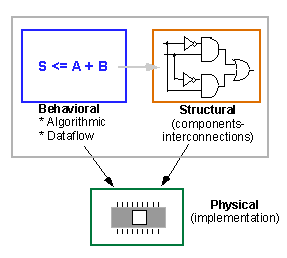
\includegraphics[width=6cm]{img/cap4/desc.png}
      \caption{Tipos de descripcion}
      \label{fig:description_types}
   \end{figure}

   \newpage
   
   Existen tres tipos basicos donde la abstracción varia dependiendo de cual se
   use, estos son:

   \begin{itemize}

      \item \textbf{Descripción comportamental: } En esta descripcion de nivel
      mas abstracto, ya que solamente describe como se comporta el circuito
      digital y solamente se tienen en cuenta las relaciones entre entradas y salidas.

      \item \textbf{Descripción de flujo de datos: } La descripción de flujo de
      datos, es la intermedia cuanto a nivel de abstracción y describe el modulo
      a partir de la prespectiva de la transformacion y transmision de datos.

      \item \textbf{Descripción estructural: } La forma de descripción
      estructural es la mas cercana a la descripcion de  una estructura real de
      hardware, ya que en esta descripcion se interconectan diferente
      componentes y puertas logicas para obtener la fucion deseada, obteniedo
      con ello el menor nivel de abstracción de los tres tipos. 

   \end{itemize}

   En la actualidad encontramos una gran cantidad de estos, no obstante
   los mas usado son VHDL y Verilog, los cuales detallaremos en el siguente
   apartado.   

   \subsection{VHDL}

      VHDL o VHSIC Hardware Description Lenguaje, es unos de los lenguajes
      dentro del estandar IEEE mas popular actualmente, que surgio en los 80 por
      parte del departamento de defensa de Estados Unidos como alternativa a los
      esquemas donde los diseñadores establecian las conexiones entre bloques,
      lo que resultaba costoso, de dificil entedimiento y poco compatibles entre
      ellos.

      \begin{figure}[h]
         \centering
         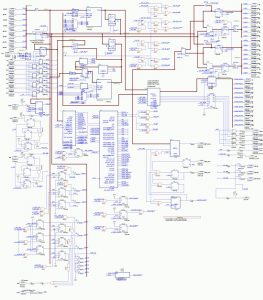
\includegraphics[width=5cm]{img/cap4/captura-esquematicos-263x300.jpg}
         \caption{Herramienta de captura de esquematicos}
         \label{fig:esquema}
      \end{figure}

      El desarollo del VHDL sutituyo al proceso anterior \ref{fig:esquema},
      consiguiendo agilizar el proceso de diseñar un diseño, hasta llegar al
      punto de ser aprobado por el comite de IEEE, siendo este ya un lenguaje
      estadarizado dentro de los estandares IEEE. 

      Como se ha comentado anteriormente, los lenguajes HDL tienen varias formas
      de describir un diseño, y VHDL puede describirlos de forma comportamental,
      estructural y de flujo de datos.  No obstante VHDL tambien permite el uso
      mixto de esto, permitiendo combinar todas las anteriores o alguna de
      ellas.

   \subsection{Verilog}

      Verilo HDL, es otro lenguaje de descripcion creado por Phil Moorby con el
      proposito de crear un lenguaje de descripcion similar a C, para que fuera
      mas familiar para el diseñador y al igual que VHDL, los dos son lenguajes
      de codigo abierto y estandarizados en la IEEE.

      Aunque Verilog, tenga similutudes en C como pueden ser algunas palabras
      reservadas y un preprocesador y los operadores de lenguaje, existen
      algunas diferencias con este, como la carencia de punteros y estructuras.
      Tambien el concepto tiempo esta en Verilog, ya que este concepto es muy
      importante en lenguajes HDL, mientras que en C no lo encontramos.

      Cuanto a su forma de describir un diseño este, solamente acepta dos formas
      de descripcion de las comentadas anteriormente, estructural y corporamental.
     
   \subsection {Metodologia de diseño} \label{md_hdl}

      Cuanto a la metodologia de diseño en lenguajes HDL encontrampos tres
      etapas, las cuales son subdividibles en otras tareas. Estas tres etapas
      son diseño logico, implementacion del diseño y finalmente verificacion del
      diseño.

      En el caso del diseño lógico, el diseñador se centra en definir el
      problema para generar los distintos diagramas de bloques, obtener las
      tablas de verdad y generar las equaciones logicas que describiran el
      corportamiento del diseño. 
      
      Una vez hemos obtenido todo lo anterior, empieza la segunda etapa, la cual
      se centra en la implementación del diseño, empezando por la seleccion del
      dispositivo, el cual lo seleccionaremos dependiendo de las necesidades de
      la implementacion, y finalmente describiremos el diseño en lenguajes
      HDL. 

      Por ultimo, quedaria la verificacion del diseño, ver si lo hecho cubre las
      necesidades y funciona correctamente. Esto se llevara a cabo mediante
      pruebas de simulacion del diseño mediante salidas esperadas dependiendo de
      la entrada dada al componente y ejecutando benchmarks, para comprobar su
      maximo potencial.  

      No obstante el diseñador puede orientar el flujo de diseño de dos formas:
      \begin{itemize}
         \item \textbf{Bottom-Up: } Esta metodología de diseño se centra en
         generar diferentes descripciones de componentes, los cuales seran
         agrupados en distintos de modulos, hasta formar un sistema completo. No
         obstante, este diseño puede llegar a ser ineficiente en diseños
         complejos y poco flexible al ser dependiente de la tecnologia usada.

         \item \textbf{Top-Down: } El diseño Top-Bottom se centra en implementar
         un diseño desde la parte de mas alto nivel e ir especificando el nivel
         de detalle segun sea necesario, esto dota al diseño de la posibilidad
         de subdividirlo en subdiseños hasta llegar a los componentes mas
         faciles de tratar y a su vez aumenta la posibilidad de reutilizar el diseño.
      \end{itemize}

      Finalmente, el diseño Top-Down proporciona mas ventajas sobre el diseño
      Bottom-Up, ya que al propio diseñador puede implementar su diseño en un
      alto nivel de abstracción o centrarse en una especifiacion mas detallada,
      lo que conlleva a ser el diseño mas utilizado.
   
\section{Register Transfer Level}

   Dentro del diseño de circuitos digitales, el Register Transfer Level o RTL es
   una capa de abstracion en el diseño de circuitos, el cual modela un circuito
   digital sincrono en cuanto a flujo de datos entre registros fisicos y
   operaciones logicas. Estos circuitos sincronos estan formadas por dos tipos
   de elementos basicos, los circuitos combinacionales, los cuales se forman a
   partir de puertas logicas y los circuitos secuenciales, los cuales se forman
   con Flip-Flop, normalmente del tipo D. 

   Esta abstracción que genera el RTL es aplicada en los lenguajes HDL, como
   Verilog o VHDL para representar el circuito en alto nivel, siendo este
   recurso muy usual en el diseño de circuitos actual. 

\section{High Level Synthesis}
   
   El High Level Synthesis o HLS es un proceso de diseño automatico, el cual
   interpreta una entrada para seguidamente transformar a esta en dispositivo
   digital que implementa el comportamiento deseado.

      \begin{figure}[h]
         \centering
         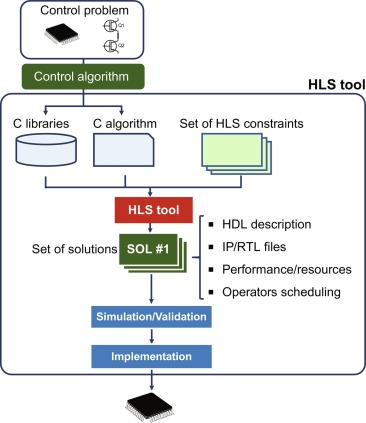
\includegraphics[width=5cm]{img/cap4/hlsprocess.jpg}
         \caption{Proceso High Level Synthesis}
         \label{fig:hls_process}
      \end{figure}

   Estas entradas suelen ser lenguajes de alto nivel, como C/C++, SystemC o
   Matlab, siendo estos analizados y limitados arquitectonicamente, para despues
   ser transcompilados a una descripcion RTL en un lenguaje HDL, que normalmente
   suelen ser VHDL o Verilog.   

   Como se ve en \ref{fig:hls_process}, el proceso del HLS consiste en un numero
   de acciones, que dependiendo de la HLS usado, siguen un orden usando 
   diferentes algoritmos y asi obtener el resultado deseado. Estas actividades son: 

   \begin{no_desc}
      \item Procesamiento lexico
      \item Optimizacion del algoritmo
      \item Analisis de control/flujo de datos
      \item Procesamiento de librerias
      \item Asignación de recursos
      \item Planificación
      \item Enlace de la unidad funcional
      \item Enlace de registro
      \item Procesamiento de salida
      \item Reagrupación de entrada 
   \end{no_desc}

   No obstante, en la actualidad los lenguajes de programacion que se usan como
   entrada, estan destinados a la interpretacion y manejo de una CPU, y esto
   provoca ciertos conflictos en el HLS a la hora de transcompilar este codigo a
   un RTL, ya que conceptos como el manejo de memoria tal y como lo conocemos en
   C/C++ no es sintetizable o la recursion, una tecnica bastante utilizada en
   algoritmos que requiera de repeticion de codigo como el Quicksort. Sin
   embargo en la actualidad existen varias empresas con su propio HLS y por lo
   cual con algunas de estas limitaciones algo diferidas enfrente otros HLS de otra
   marcas. Por tanto esta limitaciones podemos agruparlas en:

   \begin{no_desc} 
      \item Jerarquicos
      \item Sintesis de interfaces
      \item Manejo de memoria
      \item Bucle
      \item Restricciones de reloj a bajo nivel
      \item Iteracion
   \end{no_desc}

   \newpage

   \subsection{Metodologia de dise\~{n}o} \label{md_hls}

      El HLS hace el proceso de diseño mucho mas siplificado por el uso de
      lenguajes de propositos generales, como C o C++, algo mucho mas
      interiorizado actualmente y con ello reduciendo la dificultat de los
      fundamentos a numero de metodologias mucho mas amigables, que en los
      lenguajes HDL, para hacer un codigo sintetizable, esto permite que el
      proceso pueda adaptarse a metodologias de lenguajes orientados a proposito
      generales.

      \begin{figure}[h]
         \centering
         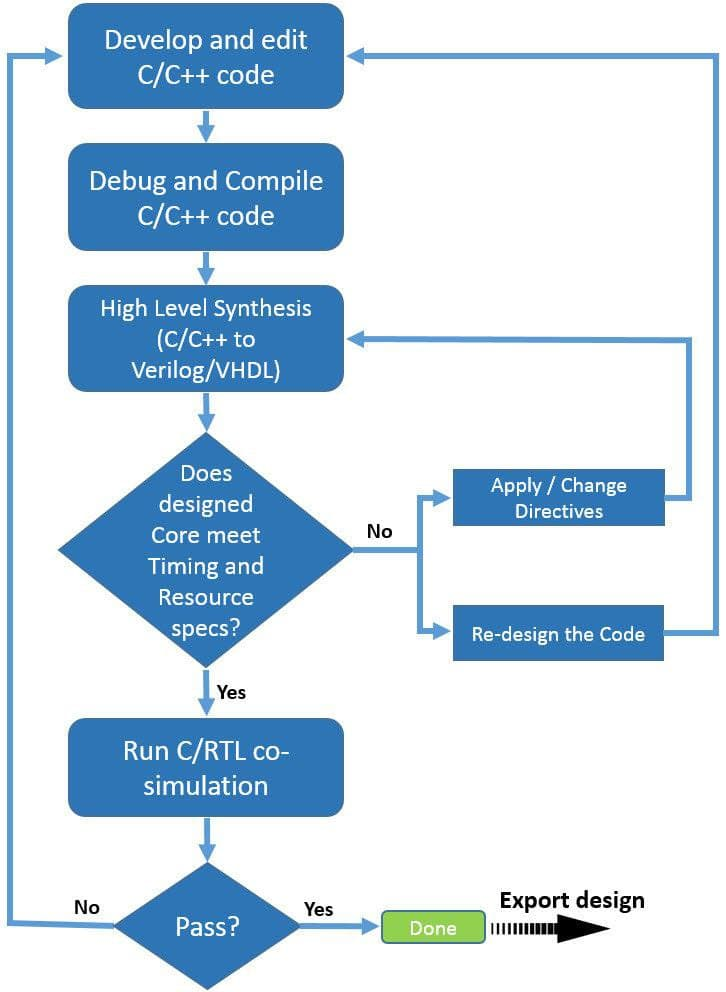
\includegraphics[width=6cm]{img/cap4/hls_design.jpg}
         \caption{Proceso de diseño en el High Level Synthesis}
         \label{fig:hls_desing}
      \end{figure}

      Como se ve \ref{fig:hls_desing}, todo el diseño se subdivide en diferentes
      etapas, la primera de todas se centra en la programacion de un codigo en
      lenguajes de proposito general y a su vez sea sintetizable, una vez
      generado esto, tenemos que comprobar si la funcionalidad de este es
      correcta mediante pruebas sin niguna tecnica para casos mas simples o para
      casos mas complejos podriamos pruebas de caja negra, ya que esta se centra
      en analizar las salidas a partir de las entradas recibidas, algo que puede
      llegar a ser util  en la etapa de depuracion y compilacion.
      
      Una vez ya este todo correcto, es hora de aplicar el HLS y comprobar si no
      genera ningun error cuanto a sintesis, sino deberiamos volver a la primera
      etapa, para generar otra solucion. En caso de pasar la sintesis, es hora
      de comprobar si el resultado dado, por el HLS es el desado en terminos de
      recursos utilizados, en caso el caso de no cumplir con lo esperado,
      tendriamos dos opciones, una seria aplicar directivas que puedan ayudar a
      optimizar partes de codigo, como dando a un arra mas de una interfaz de
      entrada o paralelizar alguno ciclos donde los datos utilizados procedan de
      lugar distino. No obstante, si las directivas no fueran capazes de generar
      un resultado que se adapte a lo deseado, tendriamos que volver a la
      primera etapa para generar otra solucion.

      Finalmente, si todo ha ido correctamente, ya solamente nos quedaria la
      ultima etapa, donde hacemos la cosimulacion de la prueba creada y el RTL
      generado, el cual podemos analizar seguidamente en un visor de ondas,
      donde veremos todas las acciones mediate ciclos de reloj. Sin embargo,
      esta simulacion puede llegar a fallar y en caso de que ocurriera, solo nos
      quedaria volver a la etapa inicial y hacer lo mismo que en los otros
      casos.

\section{Comparativa de flujo de dise\~{n}o}

   Entre los dos tipos de flujo de diseños podemos destacar ciertas
   caracteristicas que nos pueden guiar a cual usar. Algunos detalles a comparar
   podria ser:

   \subsection{Rendimiento}

      En cuanto a rendimiento, describir el diseño en lenguajes HDL, de momento
      se obtiene mayor rendimiento, ya que tratamos la problematica de forma
      especifica y aunque el HLS tambien sea una herrmaienta bastante optima a
      la hora de la generacion de RTL, esta se basa principalmente en soluciones
      generales, lo que puede llegar a mermar ligeramente el rendimiento, no
      obstante, dentro del propio HLS tiene directivas con propositos de
      optimizacion que pueden llegar a solucionar o reducir los problemas que
      puedan generar un rendimiento menor. Por tanto, la eleccion a traves de
      rendimiento, dependerá de cuanto se pueda adaptar el HLS al problema que
      queramos tratar.

   \subsection{Flexibilidad}

      En este aspecto, el High Level Synthesis ofrece mejor flexibilidad al
      cambio, ya que en esta herramienta se encarga en generar un RTL en un
      lenguaje HDL y por tanto nosotros tratamos de cambiar o corregir el codigo
      ya escrito en un lenguaje de proposito general, por tanto la tarea de
      modificar la descripcion ya hecha no es un problema a pensar, ya que el
      HLS se encargara despues de volverla a generar, mientras que en los
      lenguajes HDL, habria que pensar en una solucion y luego adaptar toda la
      descripcion a ello, lo que puede llegar a ser una labor mucho mas tardia.

   \subsection{Aprendizaje}

      Como hemos visto anteriormente, los lenguajes HDL, necesitan de ciertos
      fundamento en diseños digitales, como podrian ser los distintos tipos de
      descripciones, algo que incluso con la abstracción que aportan alguna de
      estas puede llegar a ser costoso. Sin embargo, con la herramienta HLS el
      aprendizaje es minimo y solo te basas en unas pautas para llegar a
      conseguir un codigo sintetizable en un lenguaje de proposito general, algo
      mucho mas comun en el mundo tecnolgico a dia de hoy.
\section{Conclusion}

   Finalmente, a modo de conclusion, vamos a comparar mediante la tabla
   \ref{tab:hdl_vs_hls}, las dos formas actuales de diseñar un circuito para un
   proposito, en esta tabla denotamos cual de las dos tecnologias sale ganadora
   para cada caracteristica de las tratadas en el capitulo anterior, para
   finalmente llegar a una conclusion basandonos en el coste/eficiencia.

   \begin{table}[h]
      \begin{center}
         \begin{tabular}{|l|c|c|}
            \hline
            Caracteristica & HDL & HLS \\ \hline
            Rendimiento    &  x  &     \\ \hline
            Flexibilidad   &     &  x  \\ \hline
            Aprendizaje    &     &  x  \\
            \hline
         \end{tabular}
         \caption{Conclusion lenguajes HDL vs HLS}
         \label{tab:hdl_vs_hls}
      \end{center}
   \end{table}

   Analizando la tabla desde un punto coste/eficiencia, vemos que el HLS sale
   ganador en la tabla \ref{tab:hdl_vs_hls}, ya que este tiene mas
   caracteristicas a favor que los lenguajes HDL. Esto se debe a la reduccion de
   fundamentos para poder utilizarla y su flujo de dise\~{n}o, el cual es un
   ciclo, donde el fallo redirige a la primera fase para volver a tratar el
   problema de diferente forma y dejando de lado el RTL o simplemente volver a
   tratar el problema por un posible cambio. No obstante, en cuanto al
   rendimiento, los lenguajes HLD, son mas eficiente, ya que la optimizacion es
   mas cercana a nivel bajo, cosa que el HLS es parte de la abstraccion y por
   tanto la optimizacion por el bajo nivel no esta pensada.
   
   Por tanto, mirando desde un punto coste/eficiencia el HLS es mejor opcion
   frente los lenguajes HDL.


\chapter{Vitis High-Level Synthesis}
   \section {Vitis HLS Desing Flow} %items - limitaciones, directivas, librerias 247
   \section {Advanced Micro-controller Bus Architecture}

      AMBA o ''Advanced Micro-controller Bus Architecture'', es un conjunto de 
      especificaciones de libre acceso, especializada en la comunicación entre
      bloques, que obtuvo una crecida de popularidad hasta llegar un estandar
      para la conexion, gestion y reutilizacion de bloques funcionales en SoCs.

      Aprofundizando un poco mas en el estandar AMBA, esta ofrece diversas
      caracteristacas, encontramos:

      \begin{itemize}
         \item \textbf{Flexibilidad: } Frente a la amplia variedad de SoC, con
         difrentes caracteristacas, la reutilizacion de bloques funcionales
         puede a llegar ser costosa.  Por tanto, AMBA intenta cumplir con estos
         requisitos, mediante disitintos opciones de diseño y  dotando de
         escalabidad a los procesadores compatibles. 
         \item \textbf{Adopcion generalizada: } AMBA, es actualmente el estandar
         industrial  más utilzado en los estandares basados en IP en todo el
         mundo.
         \item \textbf{Compatibilidad: } A dia de hoy, encontramos diferentes
         diseños ofrecidos por diferentes proveedores. Otorgando AMBA,
         especificaciones que aseguran compatibilidad y escalabilidad entre
         componentes IP.
         \item \textbf{Soporte: } La adopcion de las especificacion de AMBA por
         la industria ha resultado en la creacion de herramientas y productos IP
         por terceros. Gracias a esto AMBA, obtiene un amplio soporte en los
         systemas basados en sus especificaciones.
      \end{itemize}

      No obstante, en la actualidad la ultima version de AMBA, es AMBA5, sin
      emabargo Xillinx solo adopta de momento AMBA4, por tanto desarollaremos
      sus escificaciones a partir de la version que utiliza Xillinx.
      
      En cuanto a AMBA4, esta compuesta por diversas especificaciones, no
      obstante sus dos especificaciones mas desatacadas son ACE, destinada a 
      compartir datos entre componentes del sistema mediante distintos
      protocolos dedicados a la coherencia de los datos, mientras que la
      especificacion AXI, es utilizada para el desarollo de esta trabajo, la
      cual es utilizada en un amplio mercado, desde apliaciones destinadas a un
      alto rendimiento a computacion movil, redes y sector automovilístico.

      \subsection {Especificanción AXI}

         Como se ha comentado anteriormente, en este trabajo nos centraremos en
         las interfaces AXI, ya que Xillinx utiliza estas, para el manejo de los
         bloques IP. Por tanto es este apartado nos centraremos en profundizar
         en la especificacion AXI.

         La especificacion AXI o ''Advanced eXtensible Interface'', esta se une
         a AMBA en la version AMBA3 en 2003 y actualmente aun la podemos
         encontras en las versiones de AMBA4 y AMBA5.
         
         En cuanto a este, AXI es capaz de soportar diseños de alto rendimiento
         y frecuencia para efectuar las comunicaciónes de componentes de gestion
         y subordinados, ademas este es adecuado para proporcionar diseño de
         baja latencia para un amplio ancho de banda, lo que permite realizar
         diseños más rápidos, con la capacidad  funcionar en altas frequencias
         sin necesidad de crear interconexiones complejas para ello y asi poder
         conseguir bajas latencias con menor complejidad. Por otra parte AXI es
         capaz de proporcionar flexiblidad e independencia en la implementacion
         de arquitecturas de interconexion.

         Por otro lado, AXI ofrece una amplia gama de funciones, que incluyen:
         \begin{no_desc}
            \item Fases de direccion, control y datos independientes 
            \item Soporte para trasferencias de datos no alineados
            \item Solo utiliza las transaciones basadas en ''burst'', cuando 
            empiezan con una direccion inicial.
            \item Separa los canales de escritura y lectura, para activar el DMA.
            \item Capacidad para emitir multiples direciones pendientes
            \item Completado de transacciones fuera de orden
            \item Soporte para operaciones atomicas
         \end{no_desc}

         Por otra parte AXI dispone de tres interfaces mediante la version de AMBA4, 
         AXI4, AXI4-Lite, AXI4-Stream.
      
            \begin{figure}[h]
               \centering
               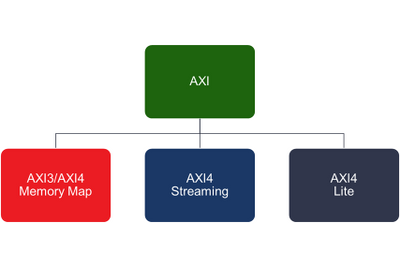
\includegraphics[width=6cm]{img/cap5/interface_types.png}
               \caption{Interfaces AXI disponibles en el HLS}
               \label{fig:hls_Interfaces}
            \end{figure}

         Cada una de estas interfaces estas destinadas a usos concretos, en el
         caso de AXI4, esta se utiliza para realizar las transferencias en
         memoria con alto rendimiento permitiendo el  ''burst'' de datos en la
         misma tranferencia, no obstante en la interfaz AXI4-Lite, esta se trata
         de una simplificación de la anterior, la cual realiza loo mismo que la
         anterior pero solamente con trasferencia simples. Por ultimo, nos queda
         la interfaz AXI4-Stream, dedicada a la transmision de alta velocidad,
         donde el maestro transfiere datos a un esclavo. 

         AXI, como se ha comentado anteriormente es un protocolo de comunicacion,
         y para ello tine definio un mecanismo de ''Handshake'', para establecer la 
         comunicacion entre el maestro y el esclavo.
         

   \section {Xillinx AXI4}

   \section {Port-level de entrada/salida}
      \subsection{No protocols}
      \subsection{Wire handshakes}
      \subsection{Memory inteface}
   \section {Block-level Protocol}
\chapter{El entorno}
   \section {Entorno de desarollo} % ide vitis
   \section {Reporte de la sintesis} % pag 68
   \section {Analizar el resultado de la sintesis} % pag 75
   \section {Waveform viewer} %pag 102
   

\chapter{Realizar una codigo sintetizable}
   \section {Limitaciones}
\chapter{Optimizacion del codigo}
\section{Directivas \#pragma}
   \section {Directivas}
\section{Librerias HLS}
      \subsection{Arbitrary Precision Data Types}
      \subsection{HLS Math}
      \subsection{HLS Video}
      \subsection{HLS IP}
      \subsection{HLS Linear Algebra}
      \subsection{HLS DSP}
\section{TMP o Template metaprograming}
\chapter{Version Final: Red neuronal}

%%%%%%%%%%%%%%%%%%%%%%%%%%%%%%%%%%%%%%%%%%%%%%%%%%%%%%%%%%%%%%%%%%%%%%%%%%%%%%%
%                                 CONCLUSIONS                                 %
%%%%%%%%%%%%%%%%%%%%%%%%%%%%%%%%%%%%%%%%%%%%%%%%%%%%%%%%%%%%%%%%%%%%%%%%%%%%%%%

\chapter{Conclusions}
https://www.legupcomputing.com/blog/index.php/benefits-of-high-level-synthesis-for-fpga-design/

%%%%%%%%%%%%%%%%%%%%%%%%%%%%%%%%%%%%%%%%%%%%%%%%%%%%%%%%%%%%%%%%%%%%%%%%%%%%%%%
%                                BIBLIOGRAFIA                                 %
%%%%%%%%%%%%%%%%%%%%%%%%%%%%%%%%%%%%%%%%%%%%%%%%%%%%%%%%%%%%%%%%%%%%%%%%%%%%%%%

\begin{thebibliography}{10}

%%%%%%%%%%%%%%%%%%%%%%%%%%%%%%%%%%%%%%%%%%%%%%%%%%%%%%%%%%%%%%%%%%%%%%%%%%%%%%%
% MODEL D'ARTICLE                                                             %
%%%%%%%%%%%%%%%%%%%%%%%%%%%%%%%%%%%%%%%%%%%%%%%%%%%%%%%%%%%%%%%%%%%%%%%%%%%%%%%
\bibitem{light}
   Jennifer~S. Light.
   \newblock When computers were women.
   \newblock \textit{Technology and Culture}, 40:3:455--483, juliol, 1999.

%%%%%%%%%%%%%%%%%%%%%%%%%%%%%%%%%%%%%%%%%%%%%%%%%%%%%%%%%%%%%%%%%%%%%%%%%%%%%%%
% MODEL DE LLIBRE                                                             %
%%%%%%%%%%%%%%%%%%%%%%%%%%%%%%%%%%%%%%%%%%%%%%%%%%%%%%%%%%%%%%%%%%%%%%%%%%%%%%%
\bibitem{ifrah}
   Georges Ifrah.
   \newblock \textit{Historia universal de las cifras}.
   \newblock Espasa Calpe, S.A., Madrid, sisena edició, 2008.

%%%%%%%%%%%%%%%%%%%%%%%%%%%%%%%%%%%%%%%%%%%%%%%%%%%%%%%%%%%%%%%%%%%%%%%%%%%%%%%
% MODEL D'URL                                                                 %
%%%%%%%%%%%%%%%%%%%%%%%%%%%%%%%%%%%%%%%%%%%%%%%%%%%%%%%%%%%%%%%%%%%%%%%%%%%%%%%
\bibitem{WAR}
   Comunicat de premsa del Departament de la Guerra, 
   emés el 16 de febrer de 1946. 
   \newblock Consultat a 
   \url{http://americanhistory.si.edu/comphist/pr1.pdf}.

\end{thebibliography}
\cleardoublepage

%%%%%%%%%%%%%%%%%%%%%%%%%%%%%%%%%%%%%%%%%%%%%%%%%%%%%%%%%%%%%%%%%%%%%%%%%%%%%%%
%                           APÈNDIXS  (Si n'hi ha!)                           %
%%%%%%%%%%%%%%%%%%%%%%%%%%%%%%%%%%%%%%%%%%%%%%%%%%%%%%%%%%%%%%%%%%%%%%%%%%%%%%%

\APPENDIX

%%%%%%%%%%%%%%%%%%%%%%%%%%%%%%%%%%%%%%%%%%%%%%%%%%%%%%%%%%%%%%%%%%%%%%%%%%%%%%%
%                         LA CONFIGURACIO DEL SISTEMA                         %
%%%%%%%%%%%%%%%%%%%%%%%%%%%%%%%%%%%%%%%%%%%%%%%%%%%%%%%%%%%%%%%%%%%%%%%%%%%%%%%

\chapter{Configuració del sistema}

????? ????????????? ????????????? ????????????? ????????????? ?????????????

\section{Fase d'inicialització}

????? ????????????? ????????????? ????????????? ????????????? ?????????????

\section{Identificació de dispositius}

????? ????????????? ????????????? ????????????? ????????????? ?????????????

%%%%%%%%%%%%%%%%%%%%%%%%%%%%%%%%%%%%%%%%%%%%%%%%%%%%%%%%%%%%%%%%%%%%%%%%%%%%%%%
%                               ALTRES  APÈNDIXS                              %
%%%%%%%%%%%%%%%%%%%%%%%%%%%%%%%%%%%%%%%%%%%%%%%%%%%%%%%%%%%%%%%%%%%%%%%%%%%%%%%


\chapter{??? ???????????? ????}

????? ????????????? ????????????? ????????????? ????????????? ????????????? 


%%%%%%%%%%%%%%%%%%%%%%%%%%%%%%%%%%%%%%%%%%%%%%%%%%%%%%%%%%%%%%%%%%%%%%%%%%%%%%%
%                              FI DEL DOCUMENT                                %
%%%%%%%%%%%%%%%%%%%%%%%%%%%%%%%%%%%%%%%%%%%%%%%%%%%%%%%%%%%%%%%%%%%%%%%%%%%%%%%

\end{document}
